\documentclass[tikz]{standalone}
\usetikzlibrary{shapes.geometric}    % trapezium
\usetikzlibrary{arrows}              % arrow tips
\usepackage{amsmath}
\usepackage{bm}                      % boldsymbol
\usepackage{makecell}                % makecell
\usetikzlibrary{matrix,calc}
\begin{document}
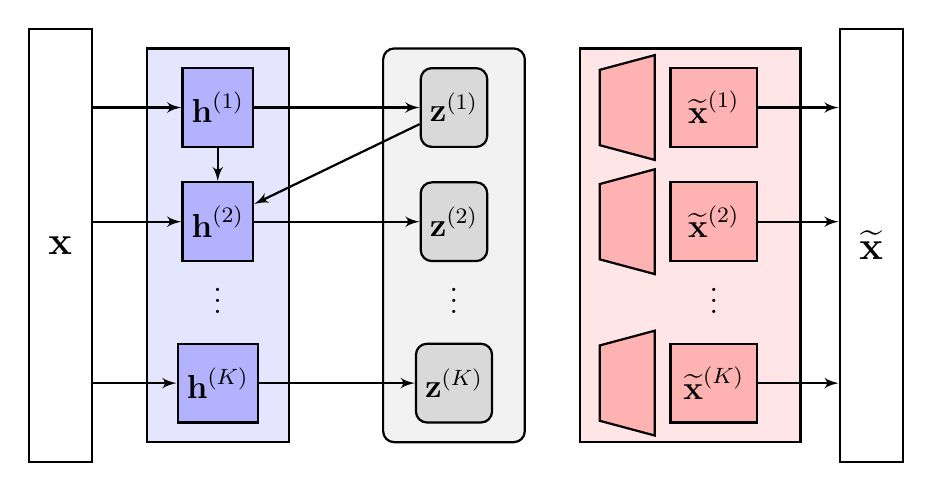
\begin{tikzpicture}[baseline=0, >=latex',thick, scale=1, every node/.style={scale=1}]
      \node (rect) at (0,0)
      [draw, thick, minimum width=0.8cm, minimum height=5.5cm, name=x] {\Large{$\textbf{x}$}};

      \node (rect) at (2, 0)
      [draw, thick, minimum width=1.8cm, minimum height=5cm, name=z, fill=blue!10] {};

      \node (rect) at (2,1.75)
      [draw, thick, minimum width=0.8cm, minimum height=1cm, name=h1, fill=blue!30]
      {\large{$\textbf{h}^{(1)}$}};

      \node (rect) at (2,0.3)
      [draw, thick, minimum width=0.8cm, minimum height=1cm, name=h2, fill=blue!30]
      {\large{$\textbf{h}^{(2)}$}};

      \node at (2,-0.6) [ minimum width=0.8cm, minimum height=0.3cm, name=hp]
      {\large{$\vdots$}};

      \node (rect) at (2,-1.75)
      [draw, thick, minimum width=0.8cm, minimum height=1cm, name=hN, fill=blue!30]
      {\large{$\textbf{h}^{(K)}$}};

      \draw [->] (h1) -- (h2);

      \draw [->] ($(x.east) + (0, 1.75)$) -- (h1.west);
      \draw [->] ($(x.east) + (0, 0.3)$) -- (h2.west);
      \draw [->] ($(x.east) + (0, -1.75)$) -- (hN.west);

      \node [rectangle, rounded corners] at (5, 0)
      [draw, thick, minimum width=1.8cm, minimum height=5cm, name=z, fill=gray!10] {};

      \node [rectangle, rounded corners] at (5,1.75)
      [draw, thick, minimum width=0.8cm, minimum height=1cm, name=z1, fill=gray!30]
      {\large{$\textbf{z}^{(1)}$}};

      \node [rectangle, rounded corners] at (5,0.3)
      [draw, thick, minimum width=0.8cm, minimum height=1cm, name=z2, fill=gray!30]
      {\large{$\textbf{z}^{(2)}$}};

      \node at (5,-0.6) [ minimum width=0.8cm, minimum height=0.3cm, name=zp]
      {\large{$\vdots$}};

      \node [rectangle, rounded corners] at (5,-1.75)
      [draw, thick, minimum width=0.8cm, minimum height=1cm, name=zN, fill=gray!30]
      {\large{$\textbf{z}^{(K)}$}};

      \draw [->] (h1) -- (z1);
      \draw [->] (z1) -- (h2);
      \draw [->] (h2) -- (z2);
      \draw [->] (hN) -- (zN);
      % \draw [->] (z2) -- ($(hp.east) + (0, -0.1)$);


      \node (rect) at (8, 0)
      [draw, thick, minimum width=2.8cm, minimum height=5cm, name=z, fill=red!10] {};

      \node [trapezium, trapezium angle=75, minimum width=1cm,
      minimum height=0.7cm,
      inner xsep=0.16cm, draw, thick, rotate=90, fill=red!30] at (7.2,1.75)
      {\rotatebox{-90}{}};

      \node (rect) at (8.3,1.75)
      [draw, thick, minimum width=1.1cm, minimum height=1cm, name=x1t, fill=red!30]
      {\large{$\widetilde{\textbf{x}}^{(1)}$}};

      \node [trapezium, trapezium angle=75, minimum width=1cm,
      minimum height=0.7cm,
      inner xsep=0.16cm, draw, thick, rotate=90, fill=red!30] at (7.2, 0.3)
      {\rotatebox{-90}{}};

      \node (rect) at (8.3,0.3)
      [draw, thick, minimum width=1.1cm, minimum height=1cm, name=x2t, fill=red!30]
      {\large{$\widetilde{\textbf{x}}^{(2)}$}};

      \node [trapezium, trapezium angle=75, minimum width=1cm,
      minimum height=0.7cm,
      inner xsep=0.16cm, draw, thick, rotate=90, fill=red!30] at (7.2, -1.75)
      {\rotatebox{-90}{}};


      \node at (8.3,-0.6) [ minimum width=0.8cm, minimum height=0.3cm, name=zp]
      {\large{$\vdots$}};

      \node (rect) at (8.3,-1.75)
      [draw, thick, minimum width=1.1cm, minimum height=1cm, name=xNt, fill=red!30]
      {\large{$\widetilde{\textbf{x}}^{(K)}$}};

      \node (rect) at (10.3,0)
      [name=xrec, draw, thick, minimum width=0.8cm, minimum height=5.5cm] {\Large{$\widetilde{\textbf{x}}$}};

      \draw [->] (x1t.east) -- ($(xrec.west) + (0, 1.75)$);
      \draw [->] (x2t.east) -- ($(xrec.west) + (0, 0.3)$);
      \draw [->] (xNt.east) -- ($(xrec.west) + (0, -1.75)$);
    \end{tikzpicture}
\end{document}
